\begin{center}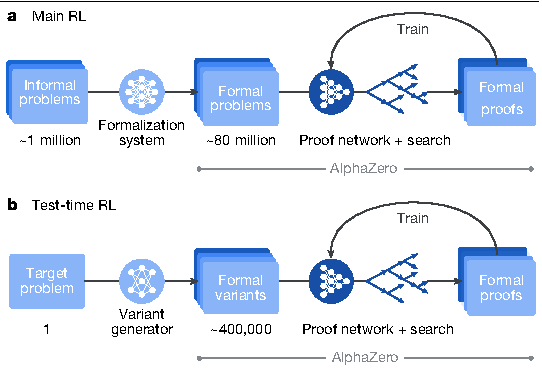
\includegraphics[width=\linewidth]{../papers/translations/alphaproof/assets/fig2.pdf}\end{center}
\phantomsection
\noindent\textbf{原文图 2. AlphaProof 的学习与适应过程.}\paperlabel{2}{alphaproof-fig2}
a, 主 RL 循环. 约 100 万非形式数学题先经形式化系统, 转为约 8000 万题的大规模形式数据集, 作为类似 AlphaZero 的 RL 课程. 证明网络结合树搜索, 在 Lean 环境生成形式证明与反证. 尝试获得的经验迭代训练、改进证明网络, 增强解答广泛问题的能力. b, TTRL 循环. 对一个具体困难形式问题, 变式生成器产生多样相关形式变式. 集中的、类似 AlphaZero 的 RL 再用证明网络与树搜索, 在这套定制变式课程上训练. 针对性学习使网络适应原题的结构和困难, 常能找到此前难以找到的形式证明. 可以同时处理多个目标. 图改编自文献\cite{alphaproof-ref28}, Google DeepMind.

\noindent\textbf{图中文字对应.} Main RL: 主强化学习; Test-time RL: 测试时强化学习; Informal problems: 非形式问题; Formalization system: 形式化系统; Formal problems: 形式问题; Proof network + search: 证明网络加搜索; Formal proofs: 形式证明; Train: 训练; Target problem: 目标问题; Variant generator: 变式生成器; Formal variants: 形式变式. 图内约 100 万、约 8000 万、1、约 400,000 等计数、AlphaZero 循环与箭头全保留原值.
